%%================= BEGIN INSTRUCTIONS =================
%%   H O W   T O   U S E   T H I S   F I L E
%% (1) download or connect to https://github.com/pmarcum/LaTex-Formatting and select the
%%        set of files (aas-style or general) that meet your situation, you can either download the files or link
%%        Overleaf to the needed files in the GitHub repository through URL, and then add the following to
%%        the preamble of your main paper
%\usepackage{FUpackages}
%\usepackage{FUformatting}
%\usepackage{FUnewCommands} % not needed by WorPT files but generally useful
%%
%% (2) copy/paste the following into the main latex file where you want to put this section of text (it is not a table), and then uncomment the below lines by removing the first percent sign at the beginning of the line
%%   IMPORTANT SHORTCUT:  You can toggle commenting / un-commenting across multiple lines within Overleaf by mouse-selecting the desired block of lines to un-comment (or comment), and then hitting: control slash ( [Ctrl] / )   ... or ...  command slash  ([command] /)  for a PC or Mac, resp.
%%        (Note that lines that should remain commented-out in the below block have 2 percent signs ... the first will be removed when you uncomment the whole block, but the second percent sign will remain as intended to retain that line as a true comment within the Latex document.)
%% > > > > > > > > > > > > > < < < < < < < < < < < < < <
%% Block of code to be uncommented by removing the *first* percent-sign at the beginning of the following lines below (leave intentional comments with at least 1 percent sign to keep them commented!)
%% The next couple of lines define cell and font colors that can be changed if desired (keep this comment line commented-out!)
%\def\myTaskTimelineColumnSize{\scriptsize } % Size of column label for Task Timeline
%\def\myTaskAssignmentsColumnSize{\scriptsize } % Size of column label for Task Assignments
%\def\myTotalFteColumnSize{\scriptsize } % Size of column label for Totaled FTEs
%\def\myYearColumnSize{\scriptsize } % Size of column label for "YR1", "YR2", etc. column labels
%\def\myTaskTitleColumnSize{\normalsize } % Size of column label for "TASK TITLES" column label
%\def\myQuarterColumnSize{\scriptsize } % Size of column label for "1", "2", "3", "4" quarter labels on columns
%\def\myIdWksColumnSize{\scriptsize } % Size of column label for "id wks"
%\def\mySigmaColumnIcon{\textbf{\large{$\Sigma$}}} % Size of Sigma symbol column label
%\def\myNoDollarColumnIcon{\noDollarIcon{-0.4}{0.4mm}{0.2}{0.15}}  % Size of "no dollar" symbol column label
%\def\myDollarColumnIcon{\dollarIcon{-0.4}{0.2}{0.015}}  % Size of "no dollar" symbol column label
%%
%\addtocounter{table}{-1} %corrects double-counting of sidewaystable and longtable combination
%\begin{sidewaystable}  %comment out if not needed
%   \begingroup
%      \setlength{\tabcolsep}{1pt}  % changes horizontal spacing between columns
%      \renewcommand{\arraystretch}{0.8} %changes vertical space between rows
%      \centerline{
%         \begin{minipage}{1.5\textwidth}  %wide table needs some of the margin?  change 1.5 to whatever
%            \begin{longtable} {|>{\raggedright\arraybackslash}p{4.1in} % title column
%               *{3}{|p{1ex}!{\color{lightgray}\vrule}*{2}{p{1ex}!{\color{lightgray}\vrule}}p{1ex}}%year
%               |>{\raggedright\arraybackslash}p{24ex}%task assignments (ID and \#Weeks)
%               |p{5ex}!{\color{lightgray}\vrule}p{5ex}!{\color{lightgray}\vrule}c|%TOTAL FTE columns
%               }
%               \expinput{do_NOT_manually_edit/NOTANONschedule}
%            \end{longtable}
%         \end{minipage}
%      }
%   \endgroup
%   \caption{\label{tab:NOTANONschedule} Resource-loaded project schedule, where: {\raisebox{-0.3\normalbaselineskip}[0pt][0pt]{
\begin{tikzpicture} \draw[fill=white,draw=red,line width=0.4mm] (0,0) circle[radius=0.2]; \draw[line width=0.4mm,red] node[midway,black]{\faDollar} (0.15,0.15) -- (-0.15,-0.15);  \draw[line width=0.4mm,red] (0.15,0.15) -- (-0.15,-0.15);  \end{tikzpicture}}} Not funded by this grant,  {\raisebox{-0.3\normalbaselineskip}[0pt][0pt]{\begin{tikzpicture}  \draw[fill=green,draw=black] (0,0) circle[radius=0.2];  \draw[draw=green] (-0.015,0.015) -- (0.015,-0.015) node[midway]{\faDollar};  \end{tikzpicture}}} funded by this grant, {\textbf{\large{$\Sigma$}}} funded $+$ unfunded; Tasks are listed (left side), with duration of task activity indicated in blue-colored timelines  that measure quarter-years (1,2,3,4). Task assignments identify specific team members responsible for  implementation with associated work weeks, where color indicates institutional affiliation  (blue$=$funded/U.S., black$=$not funded/U.S., red=international). "Total FTE" (right side) are integrated work-weeks converted into FTE per task (1~FTE$=$12~months), displayed as "total",  "unfunded by this grant", and "funded by this grant", resp.  Asignment identities:  {\textbf{dd}}: Dan.Dent{\'{o}}n, {\textbf{gg}}: Gisella.Gala, {\textbf{pm}}: Pamela.Marcum, {\textbf{ss}}: Sally.Smith}
%\end{sidewaystable}  % comment out if not used
%%================ E N D   I N S T R U C T I O N S =============== (leave this line commented out!)
\cline{2-13}
% ----------------------- First / top line of headers
\multicolumn{1}{c|}{} % title column
& \multicolumn{12}{c|}{\myTaskTimelineColumnSize {TASK}} %schedule columns
& \multicolumn{1}{c}{} %task assignment column
& \multicolumn{3}{c}{}\\ % 3-column total fte
\cline{14-17}
% ------------------------- Second line of headers
\multicolumn{1}{c|}{} % title column
& \multicolumn{12}{c|}{\myTaskTimelineColumnSize {TIMELINE}} % schedule columns
& \multicolumn{1}{c|}{\myTaskAssignmentsColumnSize {TASK}} %task assignments column
& \multicolumn{3}{c|}{\myTotalFteColumnSize {TOTAL}}\\ % 3-column total fte
\cline{2-13}
% -------------------------  Third line of headers
\multicolumn{1}{c|}{} %title column
& \multicolumn{4}{c|}{\myYearColumnSize {YR1}} & \multicolumn{4}{c|}{\myYearColumnSize {YR2}} & \multicolumn{4}{c|}{\myYearColumnSize {YR3}}
& \multicolumn{1}{c|}{\myTaskAssignmentsColumnSize {ASSIGNMENTS}} %task assignments in ID and \#week pairs
& \multicolumn{3}{c|}{\myTotalFteColumnSize {FTE}}\\ % 3-column total fte
\cline{1-1}
% -------------------------  Forth line of headers
\multicolumn{1}{|l|}{\myTaskTitleColumnSize {TASK TITLES}} % title column
& \myQuarterColumnSize {1} & \myQuarterColumnSize {2} & \myQuarterColumnSize {3} & \myQuarterColumnSize {4} %Yr1
& \myQuarterColumnSize {1} & \myQuarterColumnSize {2} & \myQuarterColumnSize {3} & \myQuarterColumnSize {4} %Yr2
& \myQuarterColumnSize {1} & \myQuarterColumnSize {2} & \myQuarterColumnSize {3} & \myQuarterColumnSize {4} %Yr3
& \multicolumn{1}{c|}{\myIdWksColumnSize {id~\#wks}} %task assignments in ID and \#week pairs
& {\textbf{\mySigmaColumnSize {$\Sigma$}}} % Col1 Total FTE
& {\myNoDollarColumnIcon } % Col2 Total FTE
& {\myDollarColumnIcon} %\Col2 Total FTE
\hline
%beginning level 1 task
{\normalsize\textbf\scshape{A}}~{\normalsize\textbf{Data and models preparation}}
& {} & {} & {} & {} & {} & {} & {} & {} & {} & {} & {} & {} % mpty year quarters
&{} %empty task assignments
&\tiny{}&\tiny{}&\tiny{}\\ %empty total FTEs
%beginning level 2 task
~{\scriptsize{\textbf{\scshape{A1}}}}~{\color{mediumelectricblue}{\footnotesize\textbf{Generate simulated data}}}
&{\tiny\cellcolor{mediumelectricblue}}&{\tiny\cellcolor{mediumelectricblue}}&{\tiny}&{\tiny}&{\tiny}&{\tiny}&{\tiny}&{\tiny}&{\tiny}&{\tiny}&{\tiny}&{\tiny}
&{ss\,8 {\small\color{blue}pm}\,{\small\color{blue}2} {\small\color{blue}dd}\,{\small\color{blue}4}}
&{\small0.27}&{\small0.04}&{\small\color{blue}0.23}\\
%beginning level 2 task
~{\scriptsize{\textbf{\scshape{A2}}}}~{\color{mediumelectricblue}{\footnotesize\textbf{Make emission maps}}}
&{\tiny\cellcolor{mediumelectricblue}}&{\tiny\cellcolor{mediumelectricblue}}&{\tiny\cellcolor{mediumelectricblue}}&{\tiny}&{\tiny}&{\tiny}&{\tiny}&{\tiny}&{\tiny}&{\tiny}&{\tiny}&{\tiny}
&{{\small\color{blue}dd}\,{\small\color{blue}6} {\small\color{blue}ss}\,{\small\color{blue}6}}
&{\small0.23}&{\small0.00}&{\small\color{blue}0.23}\\
%beginning level 2 task
~{\scriptsize{\textbf{\scshape{A3}}}}~{\color{mediumelectricblue}{\footnotesize\textbf{Incorporate thermal emission models}}}
&{\tiny}&{\tiny}&{\tiny\cellcolor{mediumelectricblue}}&{\tiny}&{\tiny}&{\tiny}&{\tiny}&{\tiny}&{\tiny}&{\tiny}&{\tiny}&{\tiny}
&{{\small\color{blue}ss}\,{\small\color{blue}6} {\small\color{black}pm}\,{\small\color{black}4}}
&{\small0.19}&{\small0.08}&{\small\color{blue}0.12}\\
\hline
%beginning level 1 task
{\normalsize\textbf\scshape{B}}~{\normalsize\textbf{Application to archive}}
& {} & {} & {} & {} & {} & {} & {} & {} & {} & {} & {} & {} % mpty year quarters
&{} %empty task assignments
&\tiny{}&\tiny{}&\tiny{}\\ %empty total FTEs
%beginning level 2 task
~{\scriptsize{\textbf{\scshape{B1}}}}~{\color{mediumelectricblue}{\footnotesize\textbf{Determine fields of interest}}}
&{\tiny}&{\tiny}&{\tiny\cellcolor{mediumelectricblue}}&{\tiny\cellcolor{mediumelectricblue}}&{\tiny\cellcolor{mediumelectricblue}}&{\tiny}&{\tiny}&{\tiny}&{\tiny}&{\tiny}&{\tiny}&{\tiny}
&{pm\,2 {\small\color{blue}dd}\,{\small\color{blue}1} {\small\color{blue}ss}\,{\small\color{blue}1} {\small\color{red}gg}\,{\small\color{red}4}}
&{\small0.15}&{\small0.12}&{\small\color{blue}0.04}\\
%beginning level 2 task
~{\scriptsize{\textbf{\scshape{B2}}}}~{\color{mediumelectricblue}{\footnotesize\textbf{Reduction of image mosaics}}}
&{\tiny}&{\tiny}&{\tiny}&{\tiny}&{\tiny\cellcolor{mediumelectricblue}}&{\tiny\cellcolor{mediumelectricblue}}&{\tiny\cellcolor{mediumelectricblue}}&{\tiny}&{\tiny}&{\tiny}&{\tiny}&{\tiny}
&{{\small\color{blue}dd}\,{\small\color{blue}4} {\small\color{blue}ss}\,{\small\color{blue}3} {\small\color{red}gg}\,{\small\color{red}5}}
&{\small0.23}&{\small0.10}&{\small\color{blue}0.13}\\
\hline
%beginning level 1 task
{\normalsize\textbf\scshape{C}}~{\normalsize\textbf{Documentation and publications}}
& {} & {} & {} & {} & {} & {} & {} & {} & {} & {} & {} & {} % mpty year quarters
&{} %empty task assignments
&\tiny{}&\tiny{}&\tiny{}\\ %empty total FTEs
%beginning level 2 task
~{\scriptsize{\textbf{\scshape{C1}}}}~{\color{mediumelectricblue}{\footnotesize\textbf{Code documentation \& verification}}}
&{\tiny}&{\tiny}&{\tiny}&{\tiny}&{\tiny}&{\tiny\cellcolor{mediumelectricblue}}&{\tiny\cellcolor{mediumelectricblue}}&{\tiny\cellcolor{mediumelectricblue}}&{\tiny\cellcolor{mediumelectricblue}}&{\tiny}&{\tiny}&{\tiny}
&{{\small\color{blue}ss}\,{\small\color{blue}8} {\small\color{blue}dd}\,{\small\color{blue}3} {\small\color{black}pm}\,{\small\color{black}6}}
&{\small0.33}&{\small0.12}&{\small\color{blue}0.21}\\
%beginning level 2 task
~{\scriptsize{\textbf{\scshape{C2}}}}~{\color{mediumelectricblue}{\footnotesize\textbf{Pub 1: pipeline and improved images}}}
&{\tiny}&{\tiny}&{\tiny}&{\tiny}&{\tiny}&{\tiny}&{\tiny}&{\tiny\cellcolor{mediumelectricblue}}&{\tiny\cellcolor{mediumelectricblue}}&{\tiny\cellcolor{mediumelectricblue}}&{\tiny}&{\tiny}
&{{\small\color{blue}dd}\,{\small\color{blue}4} {\small\color{blue}pm}\,{\small\color{blue}2} {\small\color{blue}ss}\,{\small\color{blue}4} {\small\color{red}gg}\,{\small\color{red}6}}
&{\small0.31}&{\small0.12}&{\small\color{blue}0.19}\\
%beginning level 2 task
~{\scriptsize{\textbf{\scshape{C3}}}}~{\color{mediumelectricblue}{\footnotesize\textbf{Pub 2: galaxy identification}}}
&{\tiny}&{\tiny}&{\tiny}&{\tiny}&{\tiny}&{\tiny}&{\tiny}&{\tiny}&{\tiny\cellcolor{mediumelectricblue}}&{\tiny\cellcolor{mediumelectricblue}}&{\tiny\cellcolor{mediumelectricblue}}&{\tiny\cellcolor{mediumelectricblue}}
&{{\small\color{blue}pm}\,{\small\color{blue}4} {\small\color{blue}dd}\,{\small\color{blue}3} {\small\color{blue}ss}\,{\small\color{blue}3} {\small\color{red}gg}\,{\small\color{red}6}}
&{\small0.31}&{\small0.12}&{\small\color{blue}0.19}\\
\hline